\chapter{Experimental Results} \label{C:experimental}
In this chapter the model is \textit{justified} using experimental information. Usually it is said to be the easiest part of model evaluation; whether it fits experimental measurements or not. Actually, it has been the most arduous task. Repetitive measures under different conditions, for each model, are carried out in order to validate the theoretical model.

Assumptions, simplifications and external factors made experimental results to separate from theoretical computations. Accepting this fact, the only intention is to get closer to resonant induction and be able to predict different behaviours depending on the input parameters selected.

	\section{Validations and Measurements}
In this section has been evaluated separately the resonant inductive system and the final WPT system outfitted on the drone. While in the inductive system is intended to validate the model without paying attention to the result values, in the second part these results and overall performance are discussed.


	\subsection{Resistance Estimation}
An accurate prediction of inductors' resistance is important when designing WPT systems, since it is some of the main factors that limit the power transfer capability and efficiency.

The resistance behaviour is constant until frequencies around 100 kHz. Then skin and proximity effects begin to increase the coil resistance value up to tens of ohms (\ref{F:LRvsF}). The test frequency selected to compute the theoretical values is 1 MHz. The measures on the 8 test coils are performed by using an HP 4294A Precision Impedance Analyser (40 Hz - 110 MHz). 


\begin{table}[ht]
\begin{center}
% \setlength{\tabcolsep}{12pt}
\begin{tabular}{c|c|c|r}

\noalign{\global\arrayrulewidth0.5pt}
\hline

\begin{tabular}{@{}c@{}}Coil 			\\ model 				\\								\\ $[-]$ \end{tabular} &
\begin{tabular}{@{}c@{}}Measured  		\\ resistance			\\								\\ $[\Omega]$ \end{tabular} &
\begin{tabular}{@{}c@{}}Calculated  	\\ resistance 			\\(using \ref{eq:Resistance}) 	\\ $[\Omega]$ \end{tabular} &
\begin{tabular}{@{}c@{}}Relative 		\\ error 				\\	$\epsilon_1$				\\ $[100\%]$ \end{tabular} \\

\noalign{\global\arrayrulewidth0.5pt}
\hline
\hline

$A_{Tx}$   & 0.5639 	& 	0.6519 	& 	13.49 	 	\\ \hline 
$A_{Rx}$   & 0.5916 	& 	0.6519 	& 	9.24  	 	\\ \hline 
$B_{Tx}$   & 0.6071 	& 	0.6193 	& 	2.00  	 	\\ \hline 
$B_{Rx}$   & 0.6380	 	& 	0.6193 	& 	2.93  	 	\\ \hline 
$C_{Tx}$   & 0.6704 	& 	0.6519 	& 	2.75  	 	\\ \hline 
$C_{Rx}$   & 0.6286 	& 	0.6519 	& 	3.70  		\\ \hline 
$D_{1}$    & 0.4485 	& 	0.2216 	& 	50.59 	 	\\ \hline 
$D_{2}$    & 0.3368 	& 	0.1306 	& 	61.22 		\\ \hline

\end{tabular}
\caption{Inductance calculation and measurement results}
% \label{T:K}
\end{center}
\end{table}

The results are in relatively good agreement with absolute errors smaller than 15$\%$ for the 3 candidate models. However, the theoretical resistances for models D1 and D2 are far from reality. This could be explained by the presence of AC effects when increasing frequency, and so a wrong modeling of the wire due to the varnish insulation (Table \ref{T:varnish}).




	\subsection{Inductance Estimation}
An accurate estimation of inductance is important because it is used to define the induction system model. It is also a vital parameter in tuning the resonant frequency of the WPT system. In Section \ref{subsec:coilInductance} there are defined different equations which approximate multiple-layer air-core coils.

The theoretical computations are validated through individual measures performed on the 8 test coils using an HP 4294A Precision Impedance Analyser (40 Hz - 110 MHz). The experimental values of inductance are measured in the frequency range of 10 kHz to 20 MHz. It must be said that inductance values behind 15 MHz start to behave strangely. 



\begin{table}[ht]
\begin{center}
% \setlength{\tabcolsep}{12pt}
\begin{tabular}{c|c|c|c|c|r}

\noalign{\global\arrayrulewidth0.5pt}
\hline

\begin{tabular}{@{}c@{}}Coil 			\\ model 				\\								\\ $[-]$ \end{tabular} &
\begin{tabular}{@{}c@{}}Measured  		\\ inductance			\\								\\ $[\mu\textnormal{H}]$ \end{tabular} &
\begin{tabular}{@{}c@{}}Calculated  	\\ inductance 			\\(using \ref{Eq:Wai}) 		\\ $[\mu\textnormal{H}]$ \end{tabular} &
\begin{tabular}{@{}c@{}}Relative 		\\ error 				\\	$\epsilon_1$				\\ $[100\%]$ \end{tabular} &
\begin{tabular}{@{}c@{}}Calculated  	\\ inductance  			\\(using \ref{Eq:Harold})			\\ $[\mu\textnormal{H}]$ \end{tabular} &
\begin{tabular}{@{}c@{}}Relative 		\\ error 				\\	$\epsilon_2$				\\ $[100\%]$ \end{tabular} \\

\noalign{\global\arrayrulewidth0.5pt}
\hline
\hline

$A_{Tx}$   & 12.45 	& 	12.38 	& 	0.56  	& 	11.21 	&	9.95 	\\ \hline 
$A_{Rx}$   & 12.46 	& 	12.38 	& 	0.64  	& 	11.21  	& 	10.03  	\\ \hline 
$B_{Tx}$   & 13.96 	& 	12.72 	& 	8.88  	& 	12.75 	& 	8.66  	\\ \hline 
$B_{Rx}$   & 13.7 	& 	12.72 	& 	7.15  	& 	12.75 	&	6.93 	\\ \hline 
$C_{Tx}$   & 13.67 	& 	13.26 	& 	2.99  	& 	12.60  	& 	7.82 	\\ \hline 
$C_{Rx}$   & 13.67 	& 	13.26 	& 	2.99  	& 	12.60 	& 	7.82	\\ \hline 
$D_{1}$    & 7.889 	& 	7.36 	& 	6.70  	& 	7.18  	& 	8.98  	\\ \hline 
$D_{2}$    & 4.25 	& 	4.42 	& 	4.00  	& 	4.37 	& 	2.82  	\\ \hline

\end{tabular}
\caption{Inductance calculation and measurement results}
% \label{T:K}
\end{center}
\end{table}

The results show good agreement with absolute errors smaller than 10$\%$ for Equation \ref{Eq:Wai}. The results of Equation \ref{Eq:Harold} are also quite good specially for model D2. All these computations have been performed for a test frequency of 1 Mhz. Note that inductance and resistance values are constant up to 500 kHz (see Appendix \ref{sec:RL}).


	\subsection{Quality Factor}
The experimental quality factor measurements of the coils reveal how \textit{good} the coils are for transferring energy. From Figure \ref{F:experimentalQualityFactor} it can be observed that all coils have similar Q factors, and it increases with the frequency. Hence, we will try to work at the highest possible operating frequency, which is constrained by the Equation \ref{eq:maxop}.

\begin{figure}[htb]
\begin{center}
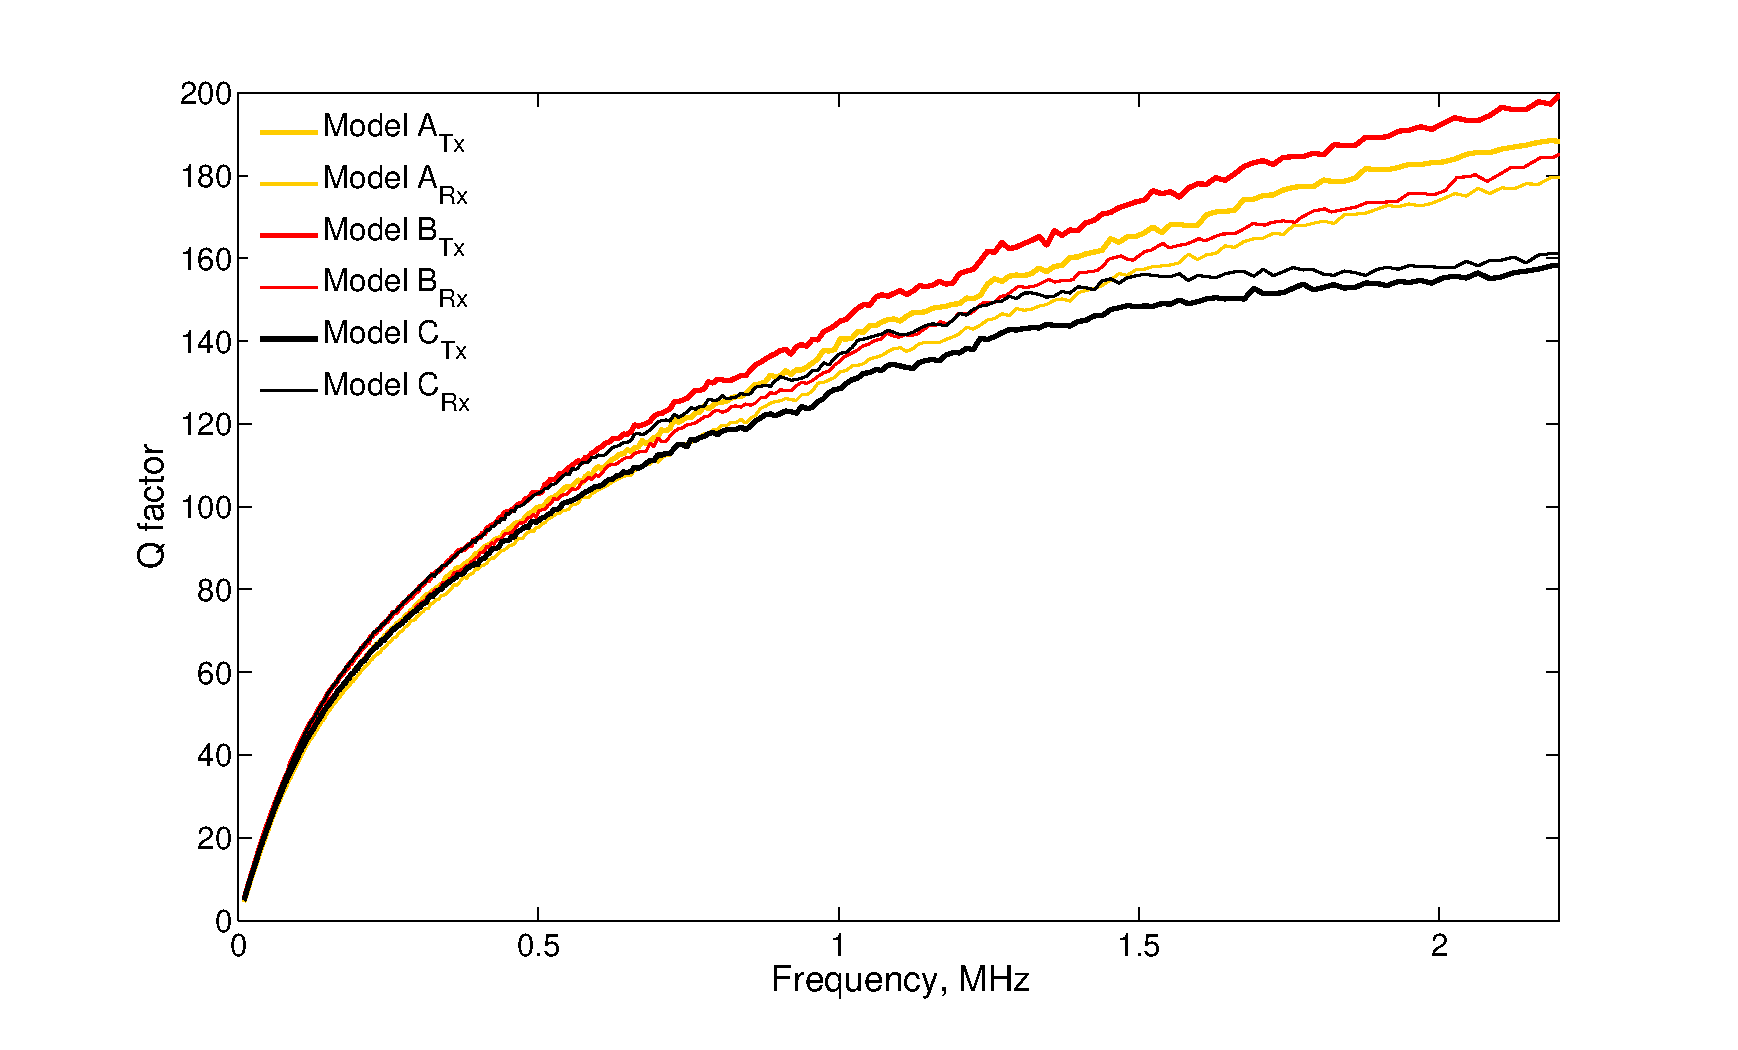
\includegraphics[width=1\textwidth]{./images/qualityFactor}
\caption{Experimental quality factor of model coils}
\label{F:experimentalQualityFactor}
\end{center}
\end{figure}

Table \ref{T:experimentalSelfFrequency} exhibits the self-resonant frequency of models A, B and C, as well as their operating frequency.

\begin{table}[htb]
\begin{center}
\begin{tabular}{c|c|c|c}

\noalign{\global\arrayrulewidth0.5pt}
\hline
Model  &   $f_s$ 	& $f_{op(max)}$ 	& Q factor\\
\hline
\hline
A      & 4.33 MHz 	 & 0.86 MHz	&      129   \\ \hline 
B      & 6.96 MHz 	 & 1.39 MHz	&      160   \\ \hline 
C      & 4.76 MHz    & 0.95 MHz&       125   \\ \hline 
\end{tabular}
\caption{Self-frequencies}
\label{T:experimentalSelfFrequency}
\end{center}
\end{table}

The Q factor values of the table above are computed for the operating frequency. It would have not been \textit{fair} to compute Q factor for the same frequency, owing to each coil has its characteristic self-resonant frequency. The complete Q factor plot with respect to the frequency is presented in Appendix \ref{F:QFactorAll}, which includes the coil models D1 and D2.


	\subsection{Inductive System Performance}
The inductive model verification and validation are performed in this part of the project. The obtained results are made with several laboratory measuring instruments that may influence in the experimental measurements. This involves the necessity of evaluate its influence in a detailed way to assure that the correct experimental value is measured.

		\subsubsection{Previous considerations}

To make the analytical measurements of the resonant inductive system and compare it with the model, it is mandatory to drive this circuit with a sinusoidal voltage source. The chosen source is the \textit{Agilent 33120A} waveform generator. This AC voltage source is selected to avoid the impedances and losses that can exist if the crystal oscillator is used as source (the overall transmission system), which its impedance and losses are more difficult to determine. Thus, the total impedance of the overall circuit depends on different stages. Working with this waveform generator we ensure having a impedance determined by the manufacturer.

The output voltage rating of the \textit{Agilent A33120A} is between 35.35 mV$rms$ to 7.071 V$rms$ and it has a fixed output impedance of 50 $\Omega$. The first important point to be taken into account is that the default setting for the function generator is to display the desired voltage as though terminated into a 50 $\Omega$ load.  As a consequence, whether the displayed voltage is set to 3.535 V$rms$, the measured voltage at the output of the generator will be of 7.071 V$rms$.

All voltage measurements are done with the \textit{Agilent DSO3062A} oscilloscope and the \textit{Agilent N2862A} probe. In this part appears the second and third important points to understand. The second one is related with the input resistance in parallel with the input capacitance of the oscilloscope probe. The problem appears when a capacitive component is measured. If this capacitance has its order of magnitude similar to the input capacitance of the oscilloscope probe (about 12 pF), the measurement may be erroneous because the input capacitance can not be negligible and they will be summed.

The last important consideration when a measurement is done is the called ``ground effect''. This effect appears when the oscilloscope is used to measure the voltage drop across a circuit element, where the probe impedance is set in parallel with this component and forces to generate another reference of the ground. The following elements will be short circuited and the displayed value on the oscilloscope will be wrong. To solve this problem, floating oscilloscopes such as \textit{Agilent U1604A} are used, allowing to cancel this ``ground effect''.

% \begin{figure}[ht!]
% 	\begin{center}
% 		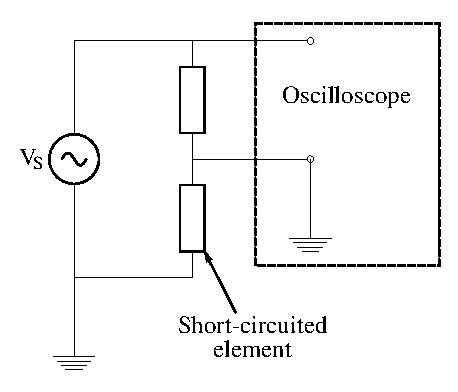
\includegraphics[width=0.7\textwidth]{./images/oscilloscope} 
% \caption{``Ground effect'' schematic}
% \label{F:GroundEf}
% 	\end{center}
% \end{figure}

		\subsubsection{Measurements methodology}

Once the previous considerations are understood, the analytical measurements can be made. In this experiment exist four independent variables which condition the measures. These variables are the source voltage, the operating frequency, the distance and the load impedance. First of all, we set the AC voltage source in 1 V$rms$ displayed (2 V$rms$ measured). The selection of this output voltage is the one to ensure that the function generator can provide the necessary power to our system without any problem. In the case that the impedance becomes small, the output current will be limited, below its maximum, by the selected low level of voltage. The measurements are made with a sinusoidal wave for three different frequencies: 0.7 MHz, 1 MHz and 2 MHz. These frequencies are selected in order to compare the behavior of the system for different sinusoidal excitations. These selection of the voltage source and the frequency leaves two independent variables defined. 

All measurements are done for SS and SP topologies for the primary and secondary coils of the same model, to simplify the comparison with the theoretical model. The optimal way to transfer energy is when the resonant frequency is the operating frequency, thus, compensation capacitors are determined depending on the operating frequency for each coil model. Two kinds of analysis are made: the efficiency and power dependence between the distance and the load impedance, the other two independent variables. This two analysis will allow us to verify the model equations for the energy transmission system, in terms of magnetic induction, and the power transferred to the secondary side, in terms of the optimal load that matches with the primary circuit.

The comparison between the real efficiency and output power with their respective theoretical values will allow us to validate the model. To perform that, first of all it is required to determine the input power. The calculation of the input power is done by computing the AC current flowing through the primary side of the core-less transformer and multiplying it by the source voltage. The calculation of an AC current is not a trivial task because typical multimeters can measure \textit{RMS} magnitudes of AC waveforms up to 300 kHz approximately. The only option for computing the AC current is to place a small resistor\footnote{The small resistor up to 1 $\Omega$ is selected not to change the behavior of the system. Large resistors could be better for determining the dropped voltage and to compute the current in a more precise way, but they will change the measured values.} in series after the source voltage and measuring, with a floating oscilloscope, the dropped voltage in this resistor; using the Ohm's law it is possible to calculate the input current. The resistor value is set to 1 $\Omega$. 

Distance analysis are made by aligning the coils concentrically. The transmission range is set from 2.5 cm to 10 cm modifying the distance each 1.25 cm. Note that this range goes from the center of the primary coil to the center of the secondary one. The selected small amplitude voltage does not allow us to increment this range. The only parameter that is variable in this case is the distance, thus, it is necessary to fix the load impedance. As it is said in Section \ref{subsec:discussion2}, the SS topology works better with small load impedances and the SP topology, with high load impedances. At the end of the Section \ref{subsec:Model} it was explained that maximum transferred power is when $Z_R$ is equal to the primary circuit impedance. Knowing that this reflected impedance is dependent on the distance and the load impedance, for each distance will be a load impedance that maximizes this power. To simplify the measures, $Z_L$ is fixed for SS and SP topologies with 75 $\Omega$ and 200 $\Omega$ respectively. In Figure \ref{F:distance} is exposed the analytical measuring procedure for a distance analysis.

The analysis with the load resistance are made by setting fixed the distance in 5 cm. For SS topology, the load is changed up to 100 $\Omega$ approximately and for SP topology, up to 7 k$\Omega$. This procedure is shown in Figure \ref{F:load}, where the two coils are distanced 5 cm.

\begin{figure}[htb]
\begin{center}
\begin{subfigmatrix}{2} 
\subfigure[Distance analysis]
{\includegraphics{./images/DistanceAnalysis}\label{F:distance}} 
\subfigure[Load analysis]
{\includegraphics{./images/LoadAnalysis}\label{F:load}}
\end{subfigmatrix}
\caption{Measuring procedure}
\label{F:procedure}
\end{center}
\end{figure}

In Appendix \ref{D1D2} it is demonstrated that an increment in \textit{Rx} radius is preferred upon the same increment in \textit{Tx} radius which was stated in Section \ref{finTFG}. This means that larger receivers allow higher power levels for a certain distance.

\subsubsection{Results}

The obtained results for all coil models are exposed in Appendix \ref{Appendix: experimental}. The distance and load resistance analysis results are quite close to the theory. The differences are due to the tolerance of the laboratory measuring instruments used. Another factor that roughly affects to the comparison between the reality and the theory is the losses due to the transmission through the air, which is the main reason of having losses. Nevertheless, the tendency of the real measures is almost the same as theoretical values curves.

	\subsection{Overall System Performance}

To complete the experimental results, the overall system performance has to be analyzed. As it has said in Chapter \ref{C:architecture}, the used coil model for the overall system is the Model C. Thus, the experimental results are obtained by analyzing some interesting points corresponding to Model C performances.

The first test was to determine the autonomy of the nano-quadcopter battery using the transmitter circuit coupled to the receiver, and charging the super capacitor without the load installed. The methodology for this test was to put the nano-quadcopter at 2.5 cm from the receiving coil using the SS topology. The full charging of the super capacitor is reached at exactly 10 minutes with the nano-quadcopter battery without being discharged. As Figure \ref{F:battery2} shows, the nano-quadcopter's  battery is completely discharged after 16 minutes approximately. The blue dashed line indicates the voltage limit where the inductive system is turned off. This limit corresponds to the minimum voltage allowed by the regulator to boost the voltage level to 12 VDC. This voltage is experimentally selected to accomplish measurable power levels in the receiver, at a distance of 20 cm.

\begin{figure}[htb]
\begin{center}
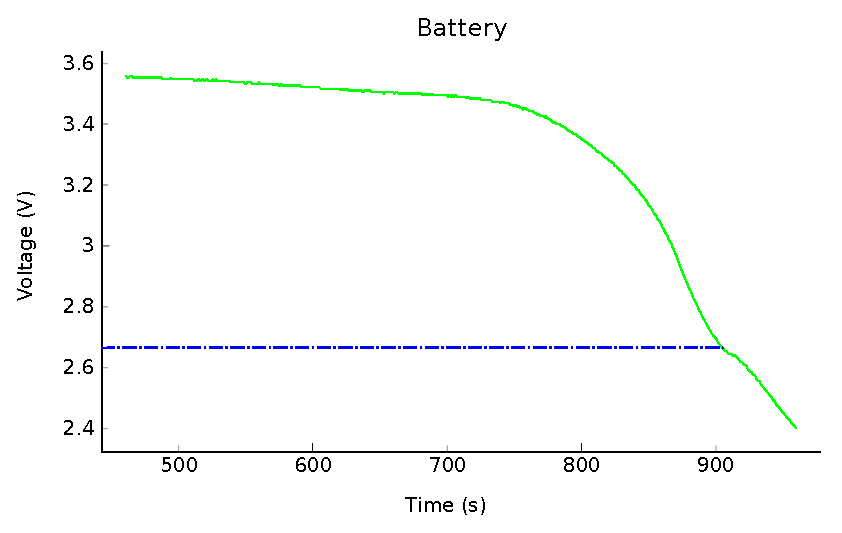
\includegraphics[width=0.8\textwidth]{./images/battery2}
\caption{Nano-quadcopter's battery discharging profile}
\label{F:battery2}
\end{center}
\end{figure}

It has been proved the same test with the SP topology and the charge time is increased over 14 minutes. The conclusion of this fact is that the load impedance (that is difficult to determine in this part of the project) could be relatively small (above 50 $\Omega$). This means that the optimal topology to use is the SS compensation topology.

Once it has tested that the nano-quadcopter can charge the super capacitor, the same experiment is done by installing the \textit{eZ430-RF2500} target board. As it has expected, the system is not able to manage the charge of the super capacitor and to run the \textit{eZ430-RF2500} at the same time. The reason is that the \textit{CC2500} RF transceiver needs to communicate with the other target board, installed on a PC for running the Sensor Monitor Visualizer Application, consuming the 21.2 mA when the battery has the equivalent energy to this current. As a result, this sensor will not communicate to its receiver and the battery will not be charged; a voltage controlled switch (like a NMOS circuit) or a push button, such as in our case, has to be implemented.

The push button (see Figure \ref{F:receiverC}) allows the nano-quadcopter to charge the battery and, when the battery is charged to the minimum voltage that can provide the enough energy for supply 21.2 mA, the push button can be triggered in order to feed the sensor. Figure \ref{F:overall} shows the realized experimental procedure for this section. In the figure it can be seen both the computer and the sensor target boards are displayed on the screen showing their temperature respectively.


\begin{figure}[H]
\begin{center}
\includegraphics[width=0.8\textwidth]{./images/overall}
\caption{Overal system measurement.}
\label{F:overall}
\end{center}
\end{figure}

Table \ref{T:finalfinal} exhibits the comparison between the theoretical and analytical power consumption.

\begin{table}[H]
\begin{center}
\begin{tabular}{c|c|c|c|c}

\noalign{\global\arrayrulewidth0.5pt}
\hline
Source voltage  &   Theoretical current & Theoretical power	& Consumed current & Consumed power 	\\
\hline
\hline
3.7 V     & 1.05 A & 3.88 W	 & 1.06 A  & 3.92 W  \\ \hline 

\end{tabular}
\caption{Consumption comparison}
\label{T:finalfinal}
\end{center}
\end{table}
